\section{Scheduling}

\mult{2}

\begin{definition}{Scheduling Problem Domain}\\
    Scheduling is a resource-time management activity:
    \begin{itemize}
        \item Focuses on managing CPU time allocation among processes
        \item Requirements vary by platform (mobile vs. supercomputer)
        \item Requirements vary by application type (batch processing vs. real-time)
    \end{itemize}
    
    Processes can be categorized by behavior:
    \begin{itemize}
        \item \textbf{CPU-bound}: Computationally intensive tasks (e.g., image processing)
        \item \textbf{I/O-bound}: Tasks that frequently wait for I/O operations (e.g., interactive applications)
    \end{itemize}
\end{definition}

\begin{concept}{When to Schedule}
    \begin{itemize}
        \item When a new process is created
        \item When a process exits
        \item When a process blocks on I/O
        \item When an I/O interrupt occurs
        \item Regularly on a timer
    \end{itemize}
    
    Based on when scheduling occurs,\\ schedulers can be:
    \begin{itemize}
        \item \textbf{Non-preemptive}: Only schedules when a process blocks or terminates
        \item \textbf{Preemptive}: Can interrupt a running process and schedule another
    \end{itemize}
\end{concept}

\begin{lemma}{Queueing Theory} base of Scheduling
    \begin{itemize}
        \item Deals with waiting for and dispatching resources
        \item Aims to provide sufficient resources to avoid under-capacity
        \item Ensures urgent tasks are not kept waiting
    \end{itemize}
\end{lemma}

\begin{theorem}{Scheduling Queues} Several Types:
    \begin{itemize}
        \item \textbf{Ready queue}: Processes waiting to be executed
        \item \textbf{Device queues}: \\ Processes waiting for specific devices
        \item \textbf{Job queue}: All processes in the system
    \end{itemize}
    
    The scheduler sorts the ready queue according to policy, and the dispatcher moves the process from the head of the queue to the CPU.
\end{theorem}

\begin{corollary}{Scheduling Metrics} used to evaluate performance:
    \begin{itemize}
        \item \textbf{CPU utilization}: \\ Keeping the CPU as busy as possible
        \item \textbf{Throughput}: \\ Number of processes completed per time unit
        \item \textbf{Turnaround time}: \\ Time from submission to completion
        \item \textbf{Waiting time}: Time spent in the ready queue
        \item \textbf{Response time}: \\ Time from request to first response
        \item \textbf{Fairness}: Equal distribution of CPU time
    \end{itemize}
\end{corollary}



\multend



\subsection{Scheduling Algorithms}

\mult{2}

\begin{definition}{Simple Schedulers}
    \begin{itemize}
        \item \textbf{Uniprocessing}: One machine, one task - no scheduler required
        \item \textbf{Multiprocessing}: Single task running at one time with job control
        \item \textbf{Multitasking}: Multiple tasks running with scheduler
    \end{itemize}
\end{definition}

\begin{concept}{Multi-level Schedulers} address priority needs:
    \begin{itemize}
        \item Multiple queues with different priorities
        \item Round Robin within each queue
        \item Challenge: High-priority tasks can cause starvation of low-priority tasks
    \end{itemize}
    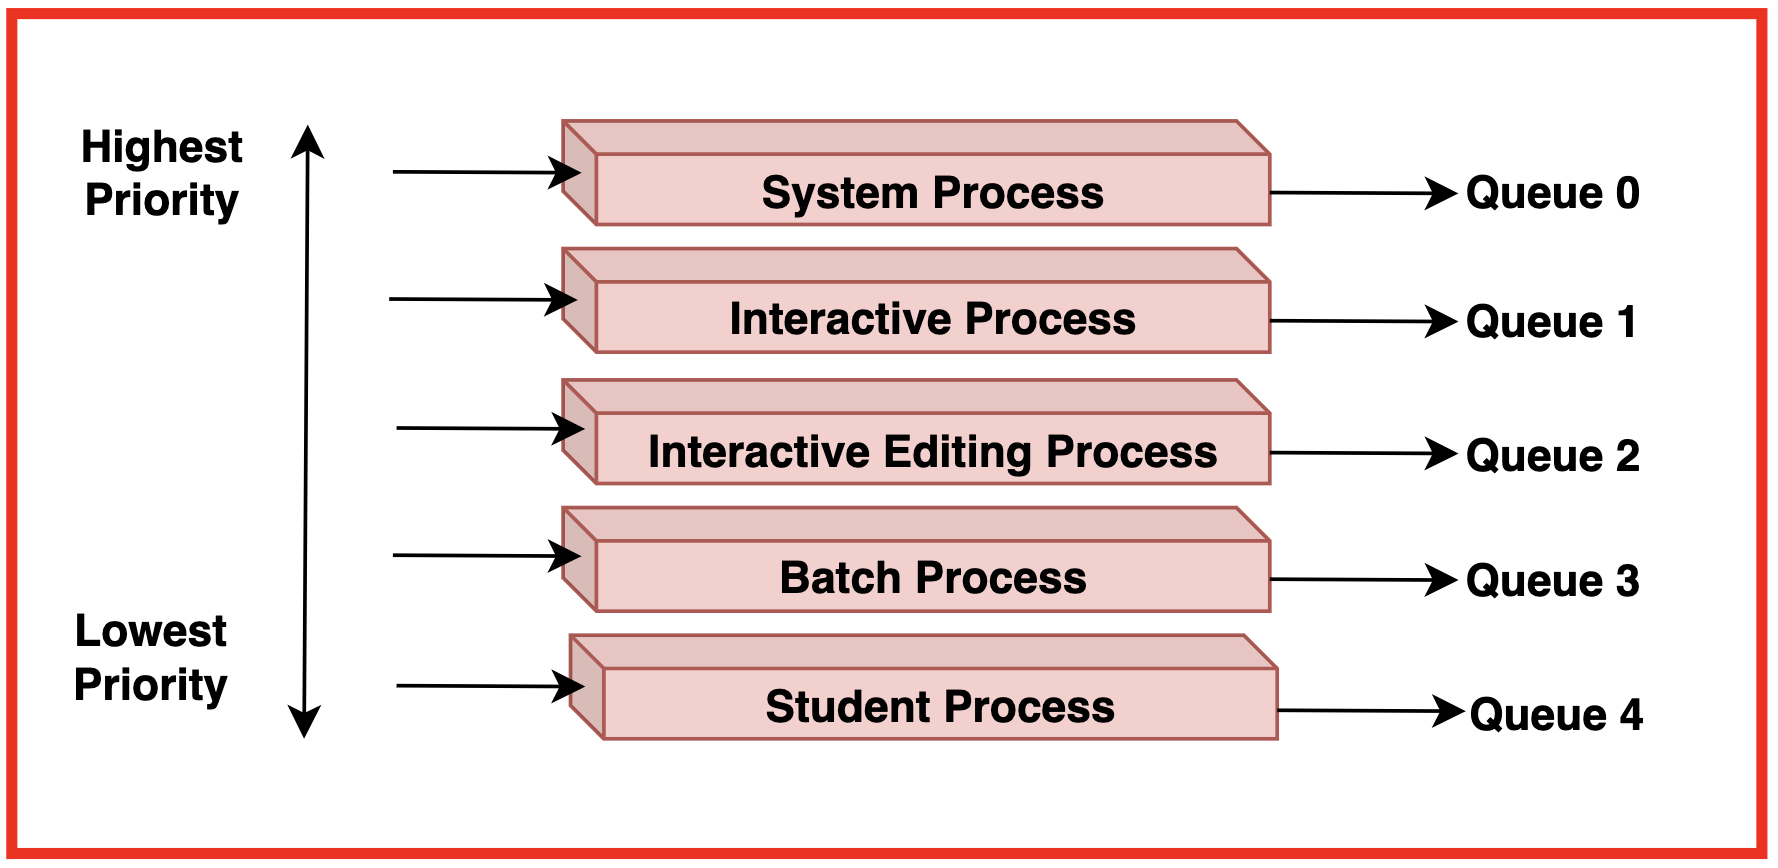
\includegraphics[width=\linewidth]{multilevel_queue.png}
\end{concept}

\begin{definition}{Fair Share Scheduling} aim for equal CPU time:
    \begin{itemize}
        \item Maintains a running clock of CPU time used per process
        \item Uses a Virtual Clock (VC) to track usage
        \item Ensures average run-time is roughly equal for all tasks
        \item Better balance between CPU-bound and I/O-bound tasks
    \end{itemize}
\end{definition}

\begin{concept}{Multi-level Feedback Queues} \\
    Addresses starvation (tasks move between queues):
    \begin{itemize}
        \item Task priority sinks after each execution interval
        \item Low-priority queues may get larger time quantum
        \item Balances responsiveness with throughput
    \end{itemize}
    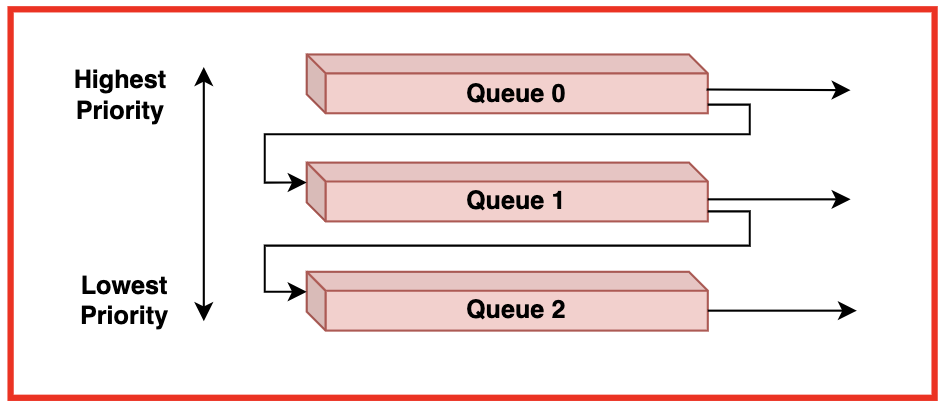
\includegraphics[width=\linewidth]{multilevel_feedback_queue.png}
\end{concept}



\multend

\mult{2}

\begin{formula}{First-In-First-Out (FIFO/FCFS)} \\ basic scheduling algorithm: 
    \begin{itemize}
        \item Processes are executed in the order they arrive
        \item Single queue, no preemption
        \item Processes run to completion
        \item Simple to implement
        \item Non-preemptive
        \item No awareness of process type (interactive vs. batch)
    \end{itemize}
    $\rightarrow$ also known as First-Come-First-Served (FCFS)

    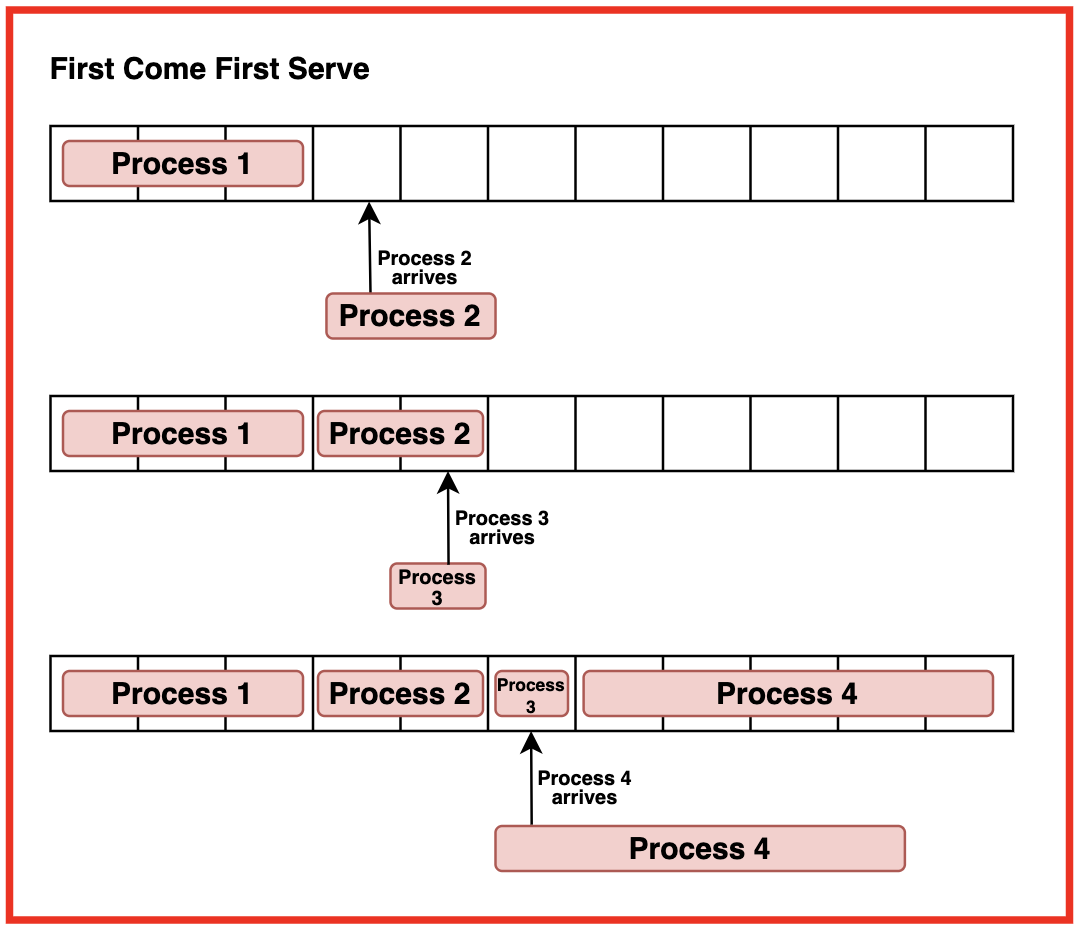
\includegraphics[width=\linewidth]{fifo_algorithm.png}
\end{formula}

\begin{formula}{Round Robin (RR)} time-sharing algorithm:
    \begin{itemize}
        \item Each process runs for a fixed time slice \\(quantum)
        \item After quantum expires, process is moved to the end of the queue
        \item Preemptive, as running tasks are interrupted after quantum
        \item Arriving tasks have priority over adjourned tasks (by convention)
        \item No starvation, as all processes eventually get CPU time
        \item Performance depends on quantum size
            \begin{itemize}
                \item Too large: approaches FIFO
                \item Too small: too much context switching overhead
            \end{itemize}
    \end{itemize}
    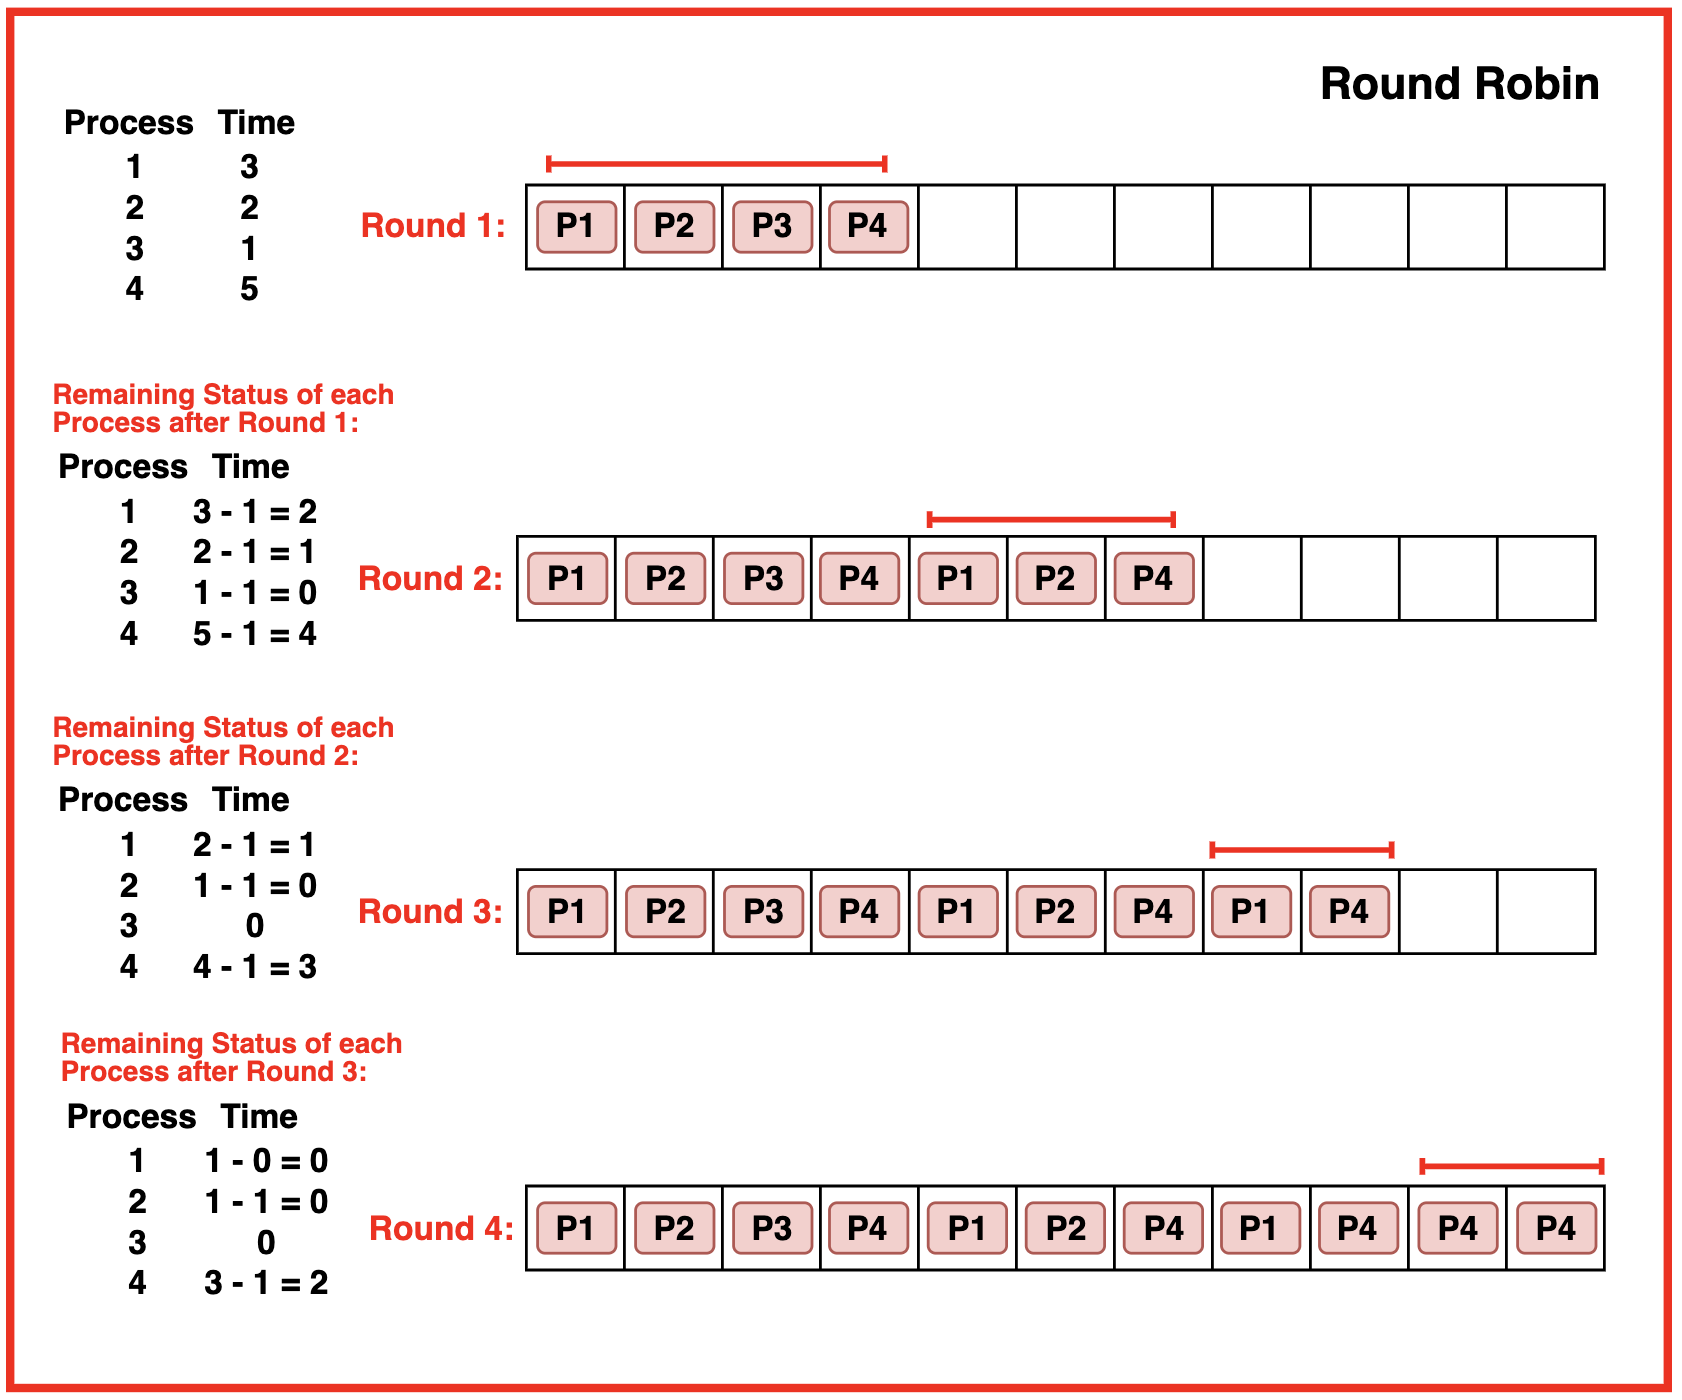
\includegraphics[width=\linewidth]{rr_algorithm.png}
\end{formula}

\begin{formula}{Shortest Job First (SJF)} \\ non-preemptive scheduling algorithm:
    \begin{itemize}
        \item Selects the process with the shortest burst time
        \item Minimizes average waiting time
        \item Non-preemptive, runs to completion
        \item Can lead to starvation for longer processes
        \item Optimal for average turnaround time
    \end{itemize}
    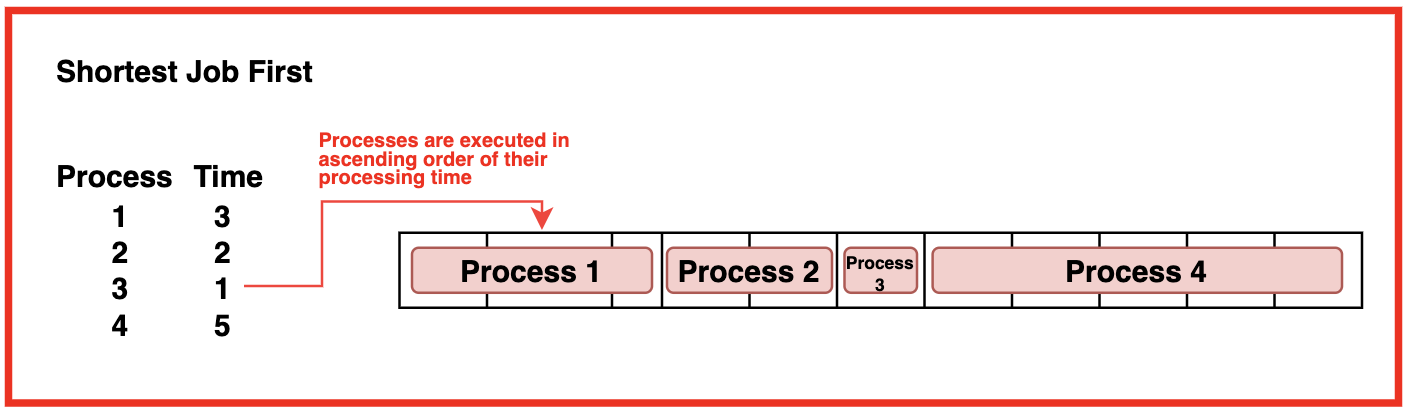
\includegraphics[width=\linewidth]{sjf_algorithm.png}
\end{formula}

\begin{formula}{Shortest Remaining Time (SRT)} \\ preemptive version of SJF:
    \begin{itemize}
        \item At each time unit, selects the process with the shortest remaining time
        \item Preempts running processes if a new process arrives with shorter remaining time
        \item Can lead to high context switching overhead
        \item Optimal for minimizing average waiting time
    \end{itemize}
   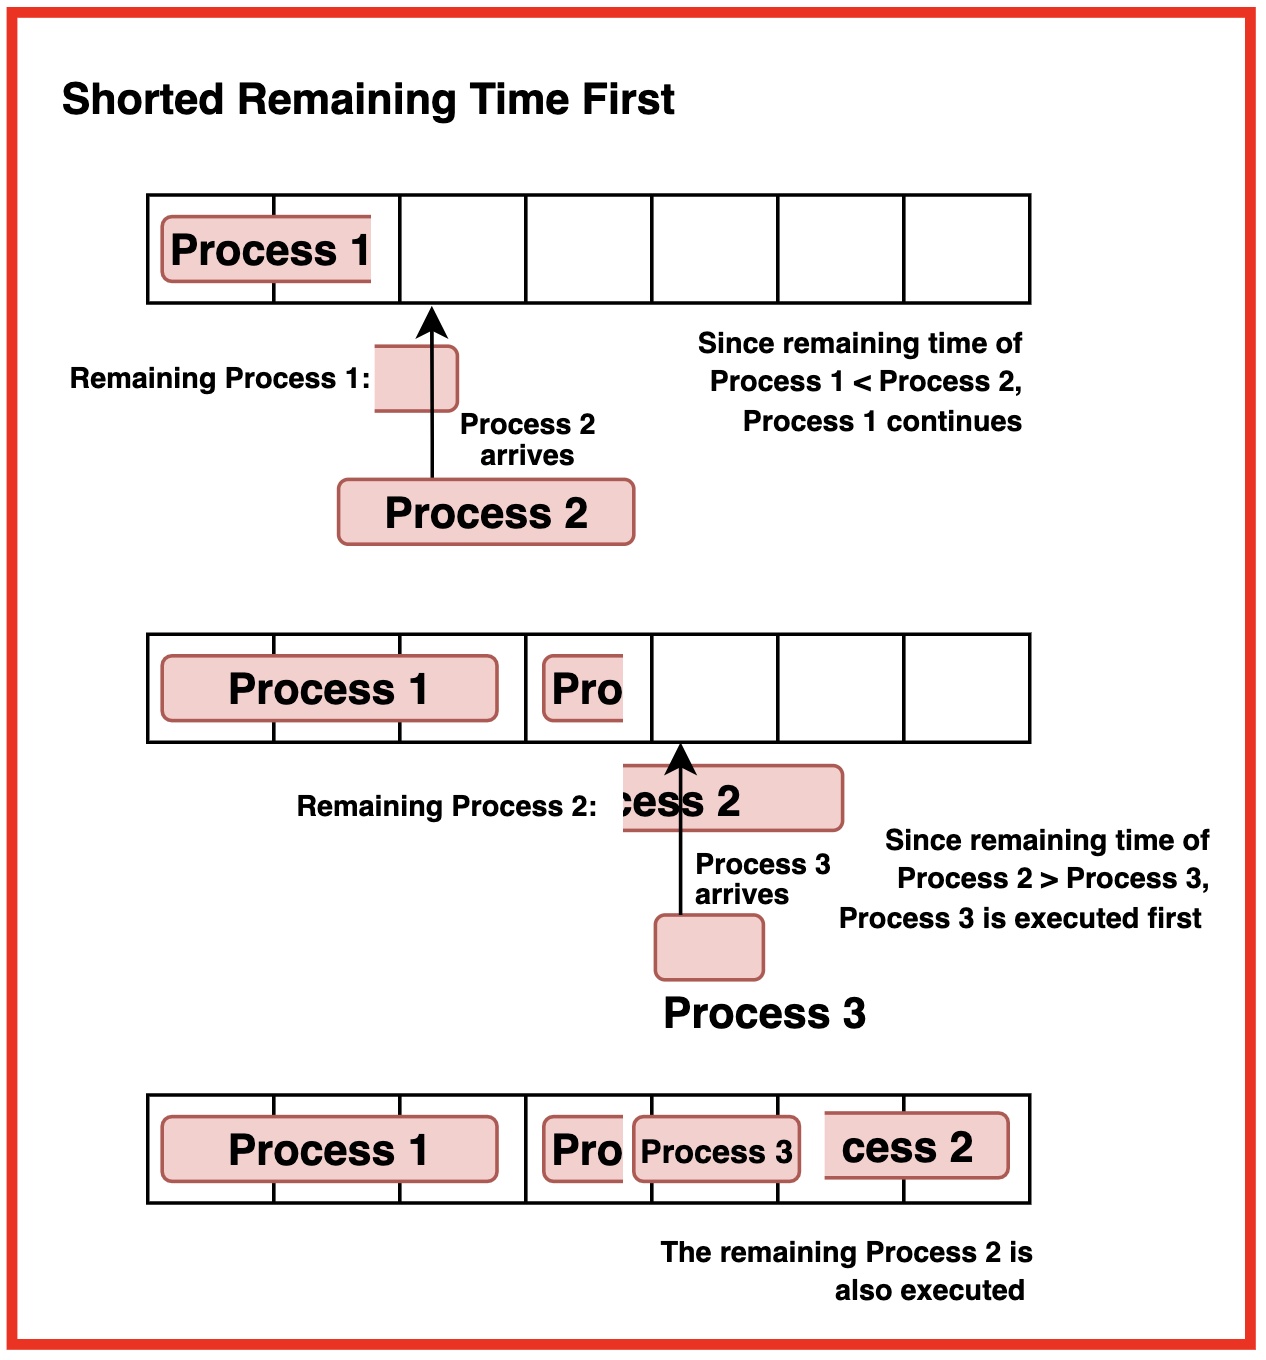
\includegraphics[width=\linewidth]{srt_algorithm.png}
\end{formula}





\begin{example2}{FIFO and RR Scheduling Comparison}\\
    Given the following task list:
    
    \begin{tabular}{|c|c|c|}
        \hline
        Task & Arrival Time & Burst Time \\
        \hline
        T1 & 0 & 10 \\
        T2 & 3 & 6 \\
        T3 & 7 & 1 \\
        T4 & 8 & 3 \\
        \hline
    \end{tabular}
    
    \textbf{FIFO Schedule}:
    
    T1 runs from 0-10, T2 runs from 10-16, T3 runs from 16-17, T4 runs from 17-20
    
    \textbf{Round Robin Schedule} (quantum = 2):
    
    T1(0-2), T1(2-4), T2(4-6), T1(6-8), T2(8-10), T3(10-11), T4(11-13), \\ T1(13-15), T2(15-17), T1(17-19), T1(19-20)
    
    RR provides better response time but potentially longer turnaround time due to context switches.
\end{example2}

\multend

\subsubsection{Scheduling Algorithm Analysis}

\mult{2}

\begin{KR}{Scheduling Algorithm Analysis}
    \paragraph{FIFO/FCFS approach}
    \begin{itemize}
        \item Execute processes in arrival order
        \item Non-preemptive
        \item Simple but may cause long wait times
    \end{itemize}
    
    \paragraph{SJF approach}
    \begin{itemize}
        \item At decision point, choose process with shortest total time
        \item Non-preemptive
        \item Optimal for average waiting time
    \end{itemize}
    
    \paragraph{SRT approach}
    \begin{itemize}
        \item At each time unit, choose process with shortest remaining time
        \item Preemptive version of SJF
        \item May cause frequent context switches
    \end{itemize}
    
    \paragraph{Problem-solving steps}
    \begin{itemize}
        \item Create timeline showing all events (arrivals, completions)
        \item For each algorithm, trace through decision points
        \item Calculate metrics: turnaround time, waiting time, response time
    \end{itemize}
\end{KR}



\begin{KR}{Round Robin Analysis}
    \paragraph{Quantum size considerations}
    \begin{itemize}
        \item Too large: Approaches FIFO, poor response time
        \item Too small: High context switching overhead
        \item Optimal: Slightly larger than typical interaction time
    \end{itemize}
    
    \paragraph{Performance factors}
    \begin{itemize}
        \item Context switch overhead
        \item Interactive response requirements
        \item CPU-bound vs. I/O-bound process mix
        \item System throughput vs. responsiveness trade-off
    \end{itemize}
\end{KR}

\begin{example2}{Round Robin Scheduling}
    Why should the time quantum be larger than typical interaction time?
    
    \textbf{Reason:}
    If the quantum is larger than interaction processing time, the entire user interaction can be completed within one quantum. This ensures the system responds quickly to user input without interrupting the interactive process.
    
    If the quantum is too small, interactive processes get interrupted before completing their response, leading to poor user experience.
\end{example2}

\multend

\begin{example2}{FIFO{,} SJF{,} and SRT Scheduling}
    Given processes with arrival and burst times, determine execution order:

    \begin{minipage}{0.35\linewidth}    
    \begin{tabular}{|c|c|c|}
        \hline
        Process & Arrival T. & Burst T. \\
        \hline
        P & 0 & 10 \\
        Q & 4 & 5 \\
        R & 5 & 10 \\
        S & 6 & 1 \\
        \hline
    \end{tabular}
    \end{minipage}
    \begin{minipage}{0.65\linewidth}    
    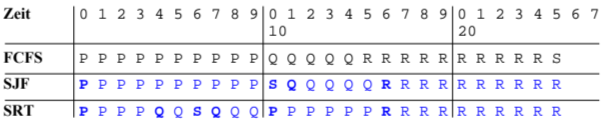
\includegraphics[width=\linewidth]{SCHEDULING_sep07.png}
    \end{minipage}
\end{example2}

\subsubsection{Multi-level Scheduling}

\begin{KR}{Priority-Based Multi-Level Scheduling}
    \paragraph{Organize by priority levels}
    \begin{itemize}
        \item Group processes by priority (higher number = higher priority)
        \item Maintain separate ready queue for each priority level
        \item Always schedule from highest priority non-empty queue
    \end{itemize}
    
    \paragraph{Apply Round Robin within priority}
    \begin{itemize}
        \item Use time quantum for processes at same priority level
        \item Move process to end of same priority queue when quantum expires
        \item New arrivals join appropriate priority queue
    \end{itemize}
    
    \paragraph{Handle preemption}
    \begin{itemize}
        \item Higher priority process always preempts lower priority
        \item Preemption occurs immediately when higher priority task arrives
        \item Preempted task returns to head of its priority queue
    \end{itemize}
\end{KR}

\begin{minipage}{0.45\linewidth}

\begin{theorem}{Priority-Based Scheduling Issues}
    \begin{itemize}
        \item Priority inversion
        \item Starvation of low-priority processes
        \item Priority assignment difficulties
        \item Real-time deadline misses
    \end{itemize}
    
    \textbf{Solution approaches:}
    \begin{itemize}
        \item Priority inheritance protocols
        \item Aging mechanisms
        \item Fair-share scheduling
        \item Deadline-based scheduling
    \end{itemize}
\end{theorem}
\end{minipage}
\begin{minipage}{0.55\linewidth}

\begin{example}
    \textbf{Priority inversion occurs when:}
    \begin{itemize}
        \item High-priority process waits for low-priority process
        \item Medium-priority processes preempt low-priority process
        \item High-priority process effectively blocked by medium-priority processes
    \end{itemize}
    
    \textbf{Prevention methods:}
    \begin{itemize}
        \item \textbf{Priority inheritance}: Low-priority process temporarily inherits high priority
        \item \textbf{Priority ceiling}: Resources assigned maximum priority of potential users
        \item \textbf{Dynamic priority adjustment}: Increase priority of waiting processes over time
    \end{itemize}
\end{example}
\end{minipage}




\begin{KR}{Multi-Level Round Robin Scheduling}

    \begin{minipage}{0.6\linewidth}
    \paragraph{Multi-level principles}
    \begin{itemize}
        \item Separate queues for different priority levels
        \item Higher priority queues are served first
        \item Round robin within each priority level
        \item Lower priority tasks only run when higher queues are empty
    \end{itemize}
    
    \paragraph{Timeline construction}
    \begin{itemize}
        \item Mark process arrivals on timeline
        \item At each time unit, determine which process should run
        \item Apply round robin within the highest non-empty priority queue
        \item Show context switches and queue changes
    \end{itemize}
    \end{minipage}
    \hspace{2mm}
    \begin{minipage}{0.35\linewidth}
    \paragraph{Scheduling algorithm}
    \begin{itemize}
        \item Group processes by priority level
        \item Always check highest priority queue first
        \item Use round robin with specified time quantum within each queue
        \item Preemption occurs when higher priority process arrives
        \item Track remaining execution time for each process
    \end{itemize}
    \end{minipage}
\end{KR}

\begin{example2}{Multi-Level Scheduling with RR}
    Five processes with time quantum = 1:
    
    \begin{minipage}{0.45\linewidth}
    \begin{tabular}{|c|c|c|c|}
        \hline
        Process & Priority & Arrival & Execution \\
        \hline
        P1 & 0 & 0 & 4 \\
        P2 & 1 & 1 & 3 \\
        P3 & 1 & 2 & 2 \\
        P4 & 0 & 5 & 3 \\
        P5 & 0 & 7 & 2 \\
        \hline
    \end{tabular}
    \end{minipage}
    \begin{minipage}{0.55\linewidth} 
    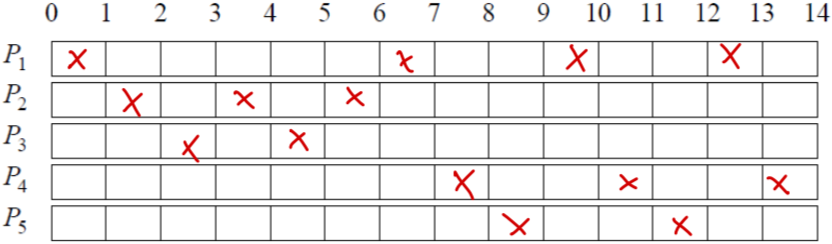
\includegraphics[width=\linewidth]{multilevelsched2.png}
    \end{minipage}
    \vspace{2mm}\\
    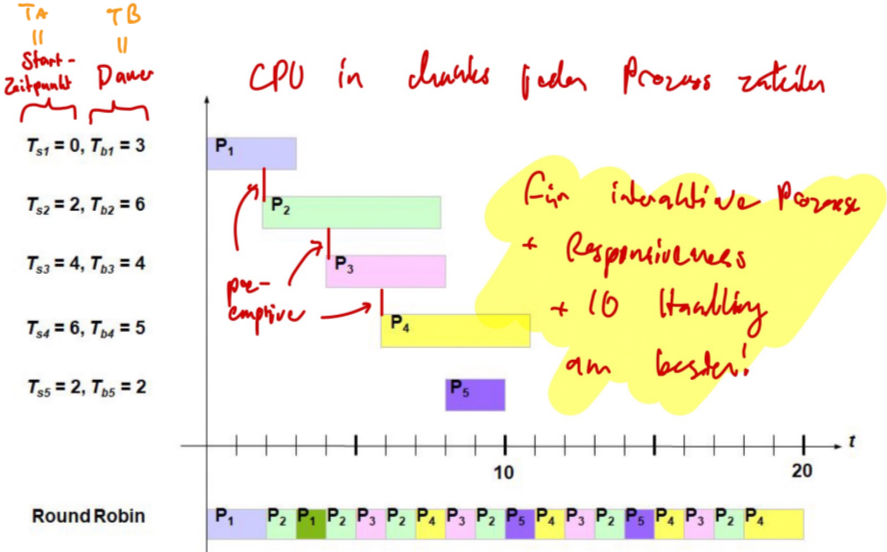
\includegraphics[width=\linewidth]{multilevel_scheduling_SEP19.png}
    \vspace{2mm}\\
    \textbf{Execution timeline:}
    \begin{itemize}
        \item t=0-1: P1 (only process available)
        \item t=1-2: P2 (higher priority, preempts P1)
        \item t=2-3: P3 (same priority as P2, P2's quantum expired)
        \item t=3-4: P2 (continues RR at priority 1)
        \item t=4-5: P3 (completes)
        \item t=5-6: P2 (completes), then P4 starts
        \item t=6-7: P1 (RR at priority 0)
        \item t=7-8: P4 (continues RR), P5 arrives
        \item And so on with RR between P1, P4, P5 at priority 0...
    \end{itemize}
\end{example2}







\subsubsection{Real-Time Schedulers}



\begin{definition}{Real-Time Systems}
    Real-time systems have specific scheduling needs:

    \begin{minipage}{0.54\linewidth}
    \begin{itemize}
        \item Need responsiveness to I/O
        \item Must fulfill deadlines (hard or soft)
        \item Hard deadlines MUST be met, soft deadlines \\can occasionally be missed
        \item Deadlines may be in milliseconds, seconds, or hours
    \end{itemize}
    \end{minipage}
    \begin{minipage}{0.45\linewidth}    
    \textbf{A Real-Time Operating System (RTOS):}
    \begin{itemize}
        \item Completes system calls in deterministic time
        \item Schedules user tasks to meet deadlines
        \item Facilitates hard real-time requirements
    \end{itemize}
    \end{minipage}
\end{definition}

\mult{2}

\begin{formula}{Rate Monotonic Scheduling}
    Static-priority \\ scheduling algorithm for real-time systems:
    \begin{itemize}
        \item Higher repetition rate tasks $\rightarrow$ higher priority 
        \item Guaranteed schedule if utilization meets criteria:
        \vspace{-2mm}\\
            $$U = \sum_{i=1}^{n} \frac{C_e}{T_r} \leq n(2^{1/n} - 1)$$
            \vspace{-2mm}\\
            \small{Where $C_e$ is execution time and $T_r$ is period}
        \item \normalsize Max. guaranteed utilization converges to \textasciitilde69\%
        \item Schedule determined at compile-time, \\ not run-time
    \end{itemize}
\end{formula}

\begin{formula}{Earliest Deadline First (EDF)}\\
    Dynamic scheduling algorithm for real-time systems:
    \begin{itemize}
        \item Scheduler determines the task with the next deadline
        \item Task with the earliest deadline gets \\ highest priority
        \item Schedule is achievable if utilization does not exceed 100\%
        \item Can achieve full CPU utilization
        \item Schedule determined at run-time, \\ not compile-time
    \end{itemize}
\end{formula}

\multend

\begin{example2}{Rate Monotonic Scheduling}
    Given tasks with the following characteristics:
    
    \begin{tabular}{|c|c|c|}
        \hline
        Task & WCET (C) & Period (T) \\
        \hline
        T1 & 10 & 20 \\
        T2 & 10 & 50 \\
        T3 & 5 & 30 \\
        \hline
    \end{tabular}
    
    \tcblower
    
    \textbf{Analysis}:\\
    1. T1 has the highest priority (shortest period)\\
    2. Utilization: $U = \frac{10}{20} + \frac{10}{50} + \frac{5}{30} = 0.5 + 0.2 + 0.167 = 0.867$\\
    3. Maximum utilization for 3 tasks: $3(2^{1/3} - 1) \approx 0.779$\\
    4. Since $0.867 > 0.779$, there is no guaranteed schedule\\    
    However, a feasible schedule might still exist. Testing would be required to confirm.
\end{example2}

\begin{example2}{Rate Monotonic Scheduling Example}\\
    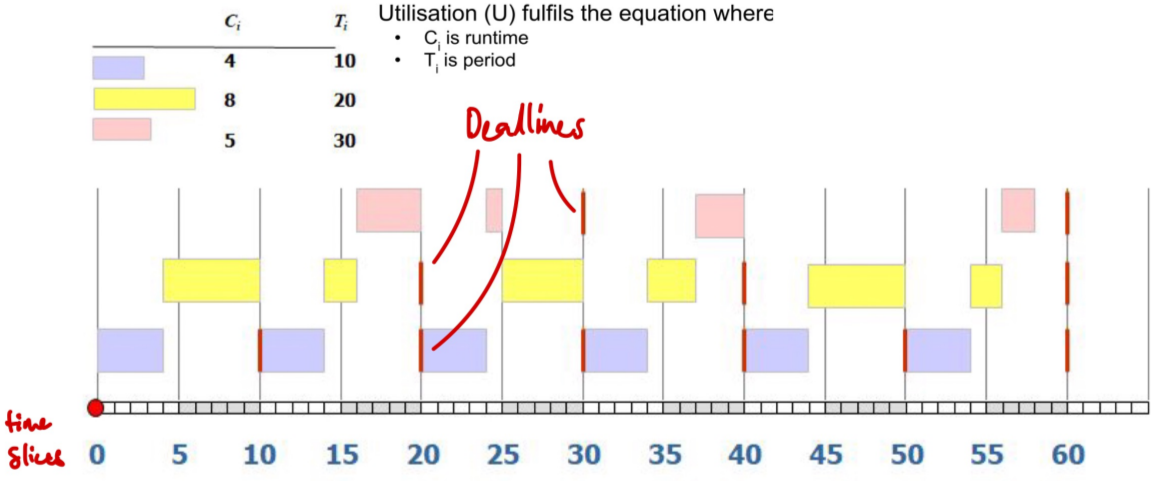
\includegraphics[width=\linewidth]{general_scheduling_example.png}
\end{example2}

\begin{minipage}{0.53\linewidth}
\begin{KR}{Earliest Deadline First Scheduling}
    \paragraph{EDF Algorithm principles}
    \begin{itemize}
        \item Always schedule the task with the earliest deadline
        \item Preemption occurs when a task with earlier deadline arrives
        \item Re-scheduling happens at specified intervals or task completion
    \end{itemize}
    
    \paragraph{Scheduling steps}
    \begin{itemize}
        \item Calculate all task deadlines for the scheduling period
        \item At each scheduling point, identify available tasks
        \item Select task with earliest deadline
        \item Handle ties with specified priority rules (e.g., shorter period)
        \item Mark execution periods in timeline diagram
    \end{itemize}
    
    \paragraph{Timeline construction}
    \begin{itemize}
        \item Create timeline with scheduling intervals marked
        \item For each interval, determine which task should run
        \item Show task execution as filled blocks
        \item Verify all deadlines are met
    \end{itemize}
\end{KR}
\end{minipage}
\begin{minipage}{0.46\linewidth}
\begin{theorem}{EDF Details}
    \paragraph{Calculating absolute deadlines}
    \begin{itemize}
        \item For each task instance:\\ Deadline = Arrival time + Period
        \item Track all active tasks \\ (arrived but not completed)
        \item Update deadlines when new instances arrive
    \end{itemize}
    
    \paragraph{Scheduling by earliest deadline}
    \begin{itemize}
        \item At each scheduling point, select task with earliest absolute deadline
        \item Preempt running task if new arrival has earlier deadline
        \item Use period as tiebreaker for equal deadlines (shorter period wins)
    \end{itemize}
    
    \paragraph{Handling rescheduling points}
    \begin{itemize}
        \item Reschedule when task completes or suspends
        \item Reschedule at fixed intervals if specified
        \item Reschedule when new task arrives \\ (if preemptive)
    \end{itemize}
\end{theorem}
\end{minipage}


\begin{example2}{EDF Scheduling}
    Three periodic tasks with rescheduling every 4ms or when a task is suspended: 
    
    \begin{tabular}{|c|c|c|}
        \hline
        Task & Period & Execution Time \\
        \hline
        \textcolor{red}{T1} & 4ms & 1ms \\
        \textcolor{red}{T2} & 8ms & 4ms \\
        \textcolor{red}{T3} & 12ms & 3ms \\
        \hline
    \end{tabular}

    Priority: in case of equal deadlines, shorter period wins.

    \tcblower
    \textbf{Preemptive Diagram:}\\
    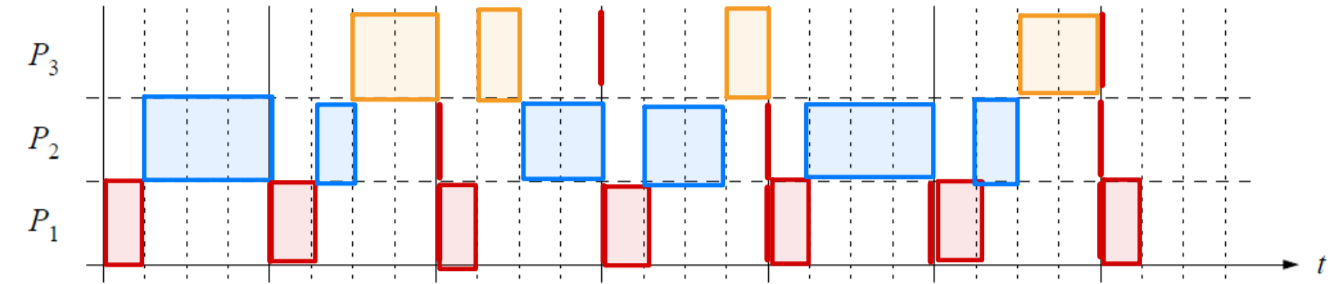
\includegraphics[width=\linewidth]{scheduling_diagram_SEP19.png}
    
    \textbf{Timeline analysis (first 24ms):}
    \begin{itemize}
        \item t=0: T1(dl=4), T2(dl=8), T3(dl=12) arrive $\rightarrow$ Schedule T1
        \item t=1: T1 completes $\rightarrow$ Schedule T2  
        \item t=4: T1(dl=8) arrives, T2 continues (dl=8, but T2 started first)
        \item t=5: T1 executes (same deadline, shorter period wins)
        \item t=6: T1 completes $\rightarrow$ Schedule T2
        \item t=8: T1(dl=12), T2(dl=16) arrive, T3 continues
        \item And so on...
    \end{itemize}
    
    The schedule ensures all deadlines are met with this task set.
\end{example2}

\raggedcolumns
\columnbreak

\subsection{Linux Scheduling}

\mult{2}

\begin{definition}{Linux Scheduling Policies}\\
    \textbf{Real-Time Policy}: For time-critical tasks
        \begin{itemize}
            \item SCHED\_DEADLINE: Earliest Deadline First + Constant Bandwidth Server
            \item SCHED\_FIFO \& SCHED\_RR (see algorithms)
        \end{itemize}
    \textbf{Normal Policy}: For regular tasks
        \begin{itemize}
            \item SCHED\_OTHER: default (CFS)
            \item SCHED\_BATCH: For batch processing tasks
            \item SCHED\_IDLE: extremely low priority bg. tasks
        \end{itemize}
\end{definition}

\begin{definition}{Linux Priority System} Kernel vs. User Space:
    \begin{itemize}
        \item \textbf{Kernel space}: Priorities from high to low
            \begin{itemize}
                \item RT: 0-99
                \item Normal: 100-139
            \end{itemize}
        \item \textbf{User space}: 'nice' values from -20 (high) to +19 (low)
            \begin{itemize}
                \item Maps to kernel priorities:\\ nice + 20 = kernel priority - 100
                \item Not used in RT policies
            \end{itemize}
    \end{itemize}
\end{definition}

\multend

\mult{2}

\begin{formula}{SCHED\_DEADLINE}
    Highest priority scheduler:
    \begin{itemize}
        \item Implements Earliest Deadline First + Constant Bandwidth Server
        \item Takes parameters: runtime, period, and deadline
        \item Tasks scheduled with this cannot fork
        \item Tasks may yield CPU time when not needed
    \end{itemize}
\end{formula}

\begin{formula}{SCHED\_FIFO}
    FIFO real-time scheduler:
    \begin{itemize}
        \item Uses one queue per priority level (1-99)
        \item Higher priority than SCHED\_RR \\ at same priority level
        \item Immediately preempts any Normal policy thread
        \item Runs to completion unless:
            \begin{itemize}
                \item Preempted by a higher priority RT thread
                \item Blocked by I/O call
                \item Voluntarily yields the CPU
            \end{itemize}
    \end{itemize}
\end{formula}

\begin{formula}{SCHED\_RR}
    Round Robin real-time scheduler:
    \begin{itemize}
        \item Similar to SCHED\_FIFO but with time quanta
        \item When quantum expires, thread moved to end of its priority queue
        \item Quantum size configurable (default 100ms)
        \item RT bandwidth limiting prevents RT tasks from monopolizing CPU
    \end{itemize}
\end{formula}

\begin{formula}{Completely Fair Scheduler (CFS)}\\
    Default scheduler in Linux (SCHED\_OTHER):
    \begin{itemize}
        \item Uses a red-black tree sorted by execution time (O(log N) operations)
        \item Tracks virtual runtime to achieve fairness
        \item Considers 'nice' values to adjust CPU share
        \item Tasks can be grouped and scheduled together
        \item Aims to model an \\ 'ideal, precise multi-tasking CPU'
        \item Time accounting managed according to configurable granularity
    \end{itemize}
\end{formula}

\begin{formula}{SCHED\_BATCH and SCHED\_IDLE}\\
    Low-priority schedulers:
    \begin{itemize}
        \item \textbf{SCHED\_BATCH}:
            \begin{itemize}
                \item Same static priority as SCHED\_OTHER
                \item Designed for batch-type, CPU-intensive tasks
                \item Applies penalty due to CPU usage
                \item SCHED\_OTHER has precedence over \\ SCHED\_BATCH at same nice value
            \end{itemize}
        \item \textbf{SCHED\_IDLE}:
            \begin{itemize}
                \item Extremely low priority
                \item Lower than static priority 0 and nice 19
                \item Used for background tasks that should only run when system is idle
            \end{itemize}
    \end{itemize}
\end{formula}

\multend

\raggedcolumns
\columnbreak

\subsection{Multi-core Scheduling}

\mult{2}

\begin{definition}{Load Balancing} on multicore systems:
    \begin{itemize}
        \item Dynamic distribution of tasks across CPU cores
        \item Applied based on scheduling policy
        \item Balances competing concerns:
            \begin{itemize}
                \item Moving tasks incurs management overhead
                \item Moving tasks incurs cache penalty \\ (lost cache advantage)
            \end{itemize}
    \end{itemize}
\end{definition}

\begin{definition}{Cache Affinity} affects scheduling decisions:
    \begin{itemize}
        \item Task data may remain in CPU cache after context switch
        \item Rerunning on the same core avoids cache misses
        \item Linux considers estimated cache live-time when migrating tasks
        \item Default cache live-time: \\ /proc/sys/kernel/sched\_migration\_cost\_ns
    \end{itemize}
\end{definition}

\multend

\begin{KR}{Analyzing Scheduling in Linux}
    \paragraph{Viewing scheduler information}
    \begin{itemize}
        \item Check process priorities: \texttt{ps -el} (PRI and NI columns)
        \item View real-time processes: \texttt{ps -eo pid,cls,pri,rtprio,nice,cmd | grep -E 'CLS|FIFO|RR'}
        \item Check scheduler statistics: \texttt{cat /proc/schedstat}
        \item See current I/O scheduler: \texttt{cat /sys/block/sda/queue/scheduler}
    \end{itemize}
    
    \paragraph{Modifying process priorities}
    \begin{itemize}
        \item Start process with nice value: \texttt{nice -n [value] command}
        \item Change nice value: \texttt{renice [value] -p [pid]}
        \item Set real-time priority: \texttt{chrt -f [priority] command} (SCHED\_FIFO)
        \item Set round-robin priority: \texttt{chrt -r [priority] command} (SCHED\_RR)
    \end{itemize}
    
    \paragraph{Analyzing schedule}
    \begin{itemize}
        \item Trace scheduling events: \texttt{trace-cmd record -e sched}
        \item View trace results: \texttt{trace-cmd report}
        \item Check CPU affinity: \texttt{taskset -p [pid]}
        \item Set CPU affinity: \texttt{taskset -c [cpu\_list] -p [pid]}
    \end{itemize}
\end{KR}




\subsubsection{Complexity Analysis}


\begin{KR}{Algorithm Complexity Analysis}
    \paragraph{Time complexity evaluation}
    \begin{itemize}
        \item O(1): Constant time, independent of input size
        \item O(log n): Logarithmic time, scales well
        \item O(n): Linear time, proportional to input size
        \item Identify bottleneck operations
    \end{itemize}
    
    \paragraph{Scheduler efficiency factors}
    \begin{itemize}
        \item Process selection time
        \item Context switch overhead
        \item Load balancing cost
        \item Priority calculation complexity
    \end{itemize}
\end{KR}

\begin{example2}{Linux O(1) Scheduler}
    Explain why the Linux O(1) scheduler is called O(1):
    
    \textbf{O(1) refers to constant time complexity:}
    \begin{itemize}
        \item Time to find next process is independent of total number of processes
        \item Uses active and expired arrays with 140 priority levels each
        \item Bitmap indicates which priority levels have waiting processes
        \item Simply finds highest priority bit set and takes first process from that queue
    \end{itemize}
    
    \textbf{Algorithm:}
    \begin{itemize}
        \item Check bitmap for highest priority with waiting processes
        \item Take first process from that priority queue
        \item Constant time regardless of system load
    \end{itemize}
\end{example2}



